\documentclass[14pt,a4paper,article]{ncc}
\usepackage[a4paper, mag=1000, left=2.5cm, right=1cm, top=2cm, bottom=2cm, headsep=0.7cm, footskip=1cm]{geometry}
\usepackage[utf8]{inputenc}
\usepackage[T2A]{fontenc}
\usepackage[english,russian]{babel}
\usepackage{indentfirst}
\usepackage{amsfonts} 
\usepackage{amssymb} 
\usepackage{amsmath, etoolbox}
\usepackage{graphicx}
\usepackage{float}
\graphicspath{{../figure/}}
\DeclareGraphicsExtensions{.png,.jpg, .jpeg}

%\bibliographystyle{gost-numeric.bbx}
\usepackage{csquotes}
\usepackage[backend=biber]{biblatex}
\addbibresource{literature.bib}

\usepackage{fancyhdr}
\pagestyle{fancy}
\fancyhead[LE,RO]{\thepage}
\fancyfoot{} 

\usepackage{listings}

%\patchcmd\subequations
%{\theparentequation\alph{equation}}
%{\subequationsformat}
%{}{}

%\newcommand{\subequationsformat}{\theparentequation.\arabic{equation}}

%\numberwithin{equation}{subsection}


\usepackage[colorlinks]{hyperref}
\hypersetup{linkcolor=black}

\begin{document}

% Title page 
\begin{titlepage}
    \begin{center}
        \textsc{
            Санкт-Петербургский политехнический университет Петра Великого \\[5mm]
            Физико-механический институт\\[2mm]
            Высшая школа прикладной математики и вычислительной физики
        }   
        \vfill
        \textbf{\large
            Компьютерные сети\\
            Отчёт по лабораторной работе №3 \\
            ``Симуляция сети с использованием протоколов SRP и OSPF'' \\[3mm]
            %по курсовой работе \\[3mm]
        }                
    \end{center}

    \vfill
    \hfill
    \begin{minipage}{0.5\textwidth}
        Выполнили: \\[2mm]   
		Студенты: Баев Даниил и Чевыкалов Григорий \\
		Группа: 5040102/30201\\
    \end{minipage}

	\hfill
	\begin{minipage}{0.5\textwidth}
		Принял: \\[2mm]
		к. ф.-м. н., доцент \\   
		Баженов Александр Николаевич
	\end{minipage}

    \vfill
    \begin{center}
        \theyear\ г.
    \end{center}
\end{titlepage}

\tableofcontents
\listoffigures
%\listoftables
\newpage

\section{Постановка задачи}
В последнее время активно развиваются проекты спутникового интернета (Starlink, OneWeb, Сфера, Бюро 1440), в основе которых лежат низкорбитальные группировки. Предлагается смоделировать связь двух наземных терминалов через спутниковую группировку. Особенностью подобных группировок является использование низких орбит, что приводит к тому, что в зоне видимости терминалов постоянно находятся разные спутники, так же это осложняет связь между самими спутниками. Это делается для большего покрытия (связь со спутником на геостационарной орбите невозможна для терминала выше восьмидесятой параллели) и для меньших задержек. Ставится задача моделирования связи двух терминалов через такую группировку.

\section{Теория}
Для моделирования движения спутников используется простейшая модель, не учитывающая торможение и другие возмущения. По Кеплеровским элементам орбиты (большая полуось, эксцентриситет, наклонение, долгота восходящего узла, аргумент перицентра, средняя аномалия) в момент $t_0$ предсказывается положение спутника в момент времени $t$.

Наличие связи между спутниками определяется по предельному углу (чтобы Земля не перекрывала линию прямой видимости). Связь между спутником и терминалом так же определяется по углу (ограниченному, чтобы избежать связи со спутником слишком близким к горизонту).

Для нахождения оптимального пути между терминалами используется протокол Open Shortest Path First, учитывающий расстояние между элементами сети. Для симуляции передачи данных используется протокол Selective Repeat. 



\section{Реализация}
Приложение реализовано на языке Python с использованием библиотек Panda3d и NetworkX. Поддерживается загрузка конфигурации спутниковой группировки и терминалов. Пример конфигурации:

\begin{verbatim}
{
    "camera_rotation_angle": 0,
    "camera_rotation_angle_vertical": 0,
    "camera_radius": 40,
    "dash_cone_angle": 65,
    "time_factor": 500.0,
    "update_topology_interval": 0.1,
    "sending_interval": 0.05,
    "loss_probability": 0.2,
    "window_size": 8,
    "timeout": 0.5,
    "sprite_size": 0.5,
    "num_orbit_segments": 1000,
    "orbit_color": [1, 1, 1, 0.8],
    "orbit_thickness": 1.5,
    "path_color": [0, 1, 0, 0.8],
    "path_thickness": 1.5,
    "dashes": [
        {
            "lat": 56.85,
            "long": 60.61
        },
        {
            "lat": 40.42,
            "long": -74.00
        }
    ],
    "satellites": [
        {
                "a": 26.6,
                "e": 0.74,
                "i": 63.4,
                "omega": 0,
                "w": 90,
                "m": 270
        },
        {
                "a": 26.6,
                "e": 0.74,
                "i": 63.4,
                "omega": 90,
                "w": 90,
                "m": 90
        }
    ]
}
\end{verbatim}
\newpage
Управление началом передачи осуществляется через форму.

\begin{figure}[H]
    \centering
    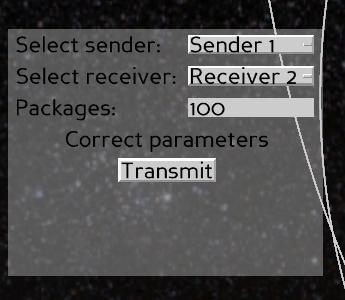
\includegraphics[width=0.5\linewidth]{form.png}
    \caption{Форма управления}
    \label{fig:form}
\end{figure}

Терминалы отображаются в виде ''спутниковой тарелки'', спутники в виде соответствующего значка.

\begin{figure}[H]
    \centering
    
\includegraphics[width=0.25\linewidth]{satellite-dash.png}
    \caption{Обозначение терминала}
    \label{fig:dash}
\end{figure}

\begin{figure}[H]
    \centering
    
\includegraphics[width=0.25\linewidth]{satellite.png}
    \caption{Обозначение спутника}
    \label{fig:satellite}
\end{figure}

Вращение камеры осуществляется мышью. При передаче данных путь передачи отображается зеленой линией.

\section{Результаты}
Были протестированы различные конфигурации группировки (аналог ''молнии'' и ''OneWeb''). Низкоорбитальные группировки обеспечивают хорошее покрытие и низкую задержку, однако поддержка актуального графа является сложной задачей.

\begin{figure}[H]
    \centering
    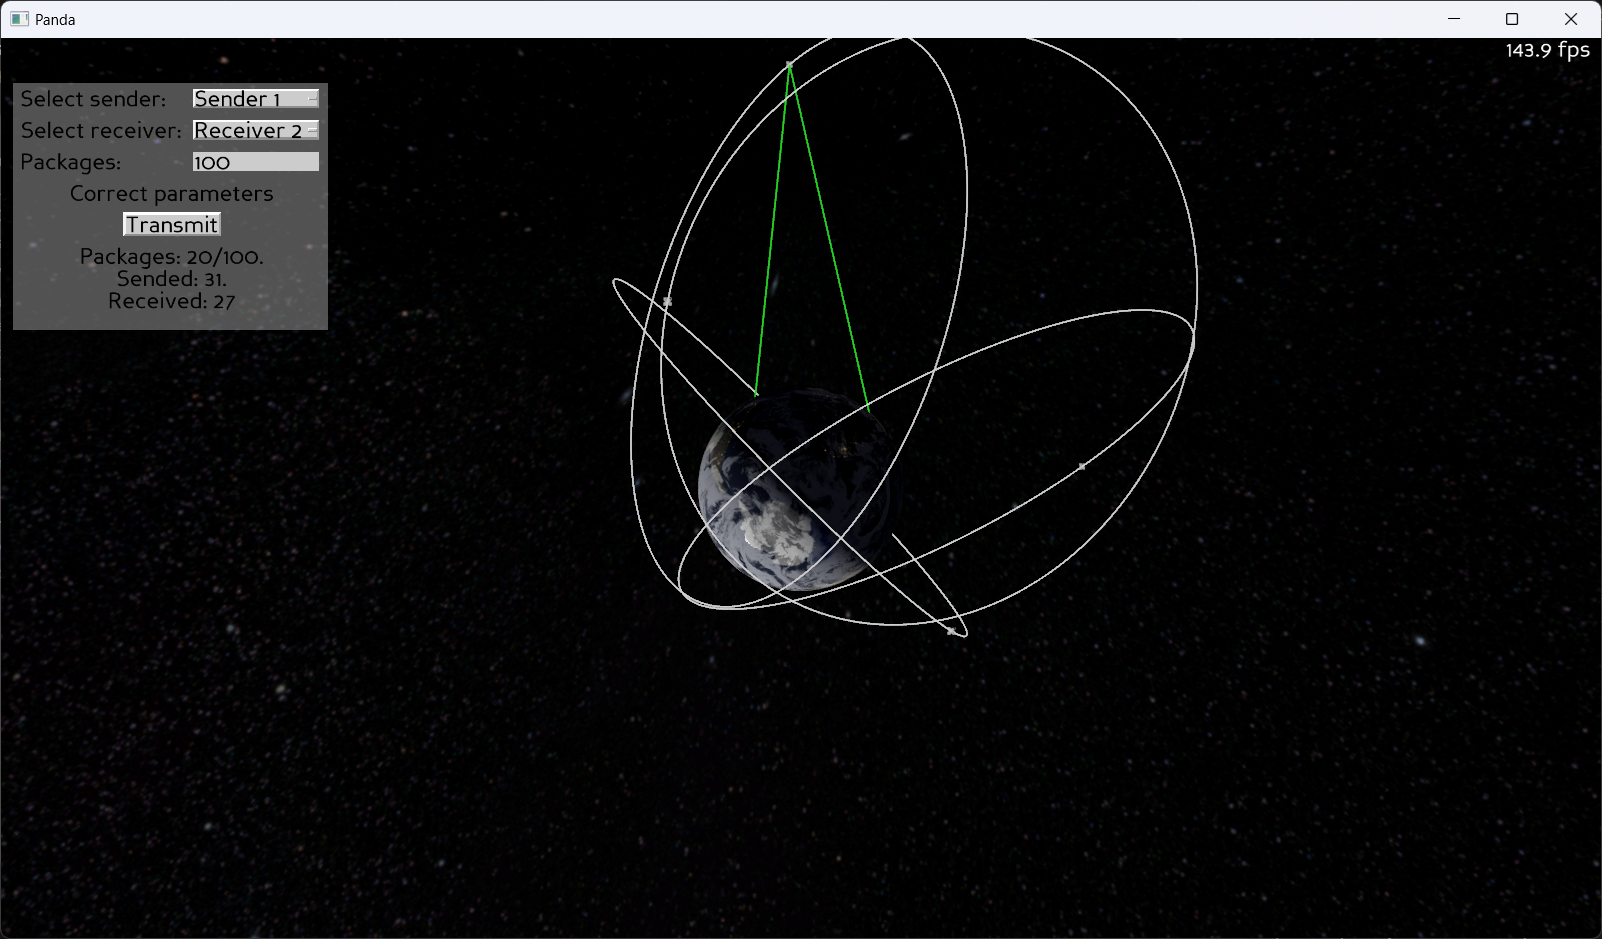
\includegraphics[width=0.9\linewidth]{image_1.png}
    \caption{Пример работы для аналога конфигурации ''молния''}
    \label{fig:image_1}
\end{figure}

\begin{figure}[H]
    \centering
    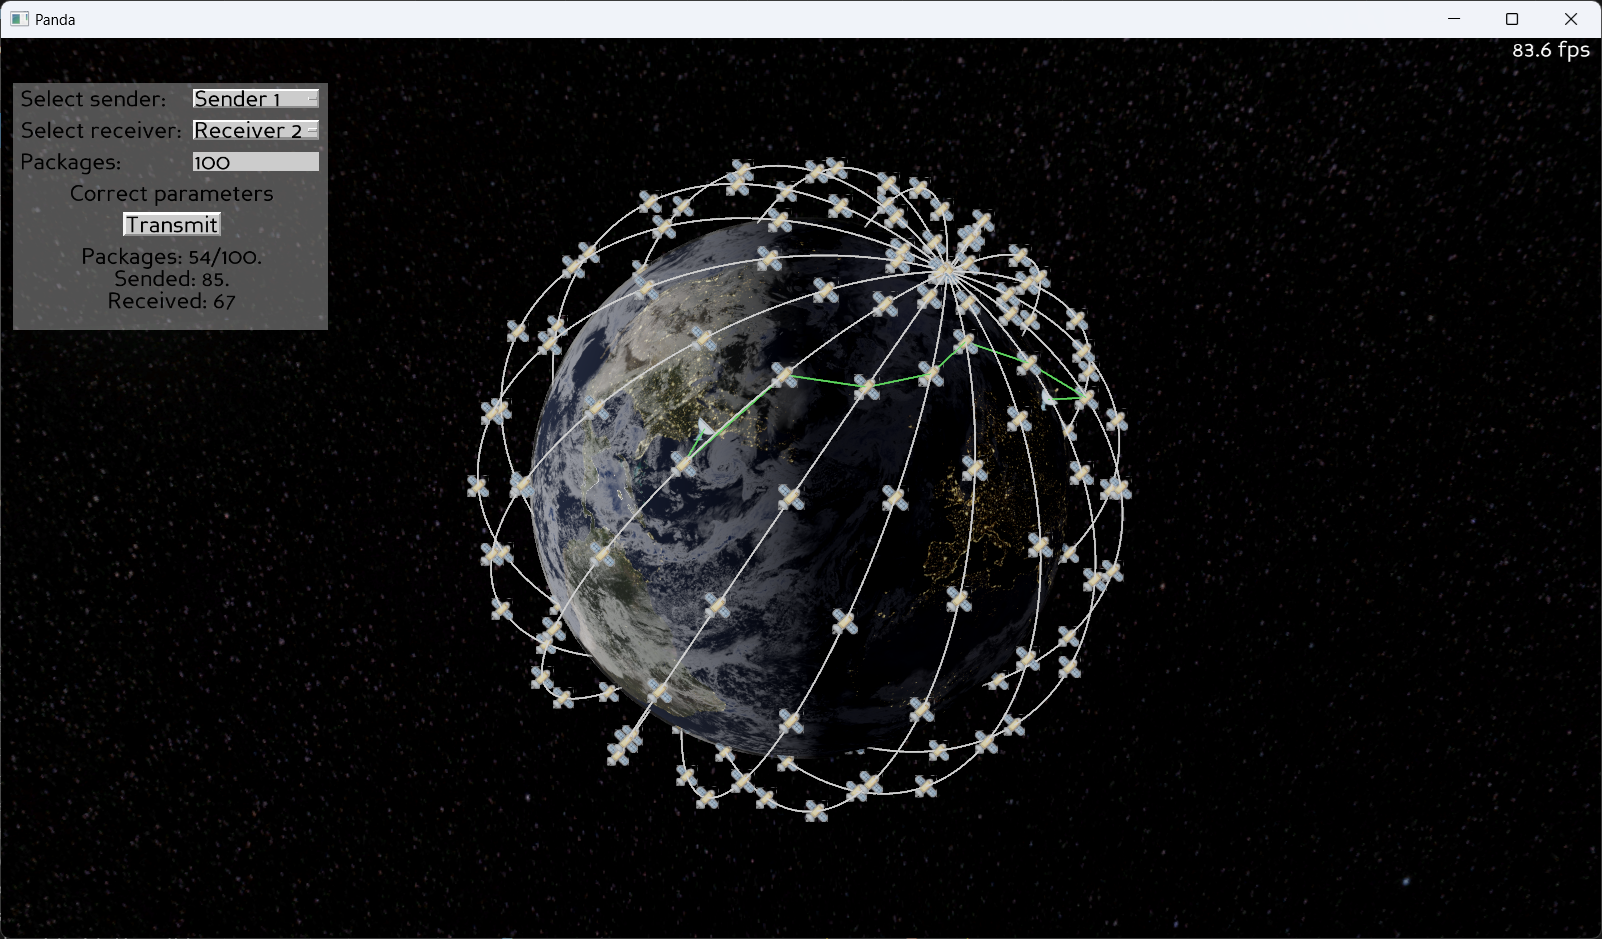
\includegraphics[width=0.9\linewidth]{image_2.png}
    \caption{Пример работы для аналога конфигурации ''OneWeb''}
    \label{fig:image_2}
\end{figure}

\section{Обсуждение}
В результате работы создано приложение, использующее протоколы Selective Repeat и Open Shortest Path First для симуляции связи через спутниковый интернет, поддерживающей порядка ста спутников. Благодаря использованию этих алгоритмов есть возможность перестройки сети при постоянном перемещении спутников по орбитам.

\printbibliography
%\addcontentsline{toc}{section}{Литература}

\section{Приложения} \label{app}

\begin{enumerate}
	\item Репозиторий с кодом программы и кодом отчёта:
	
	\href{https://github.com/CurveCube/Networks_coursework}{https://github.com/CurveCube/Networks-coursework}

\end{enumerate}


\end{document}
